\BourbakiUnnumberedChapter{Historical Note}{Historical Note (Chapters IV and V)}

(Chapters IV and V)

(Numbers in brackets refer to the bibliography at the end of this Note.)

The theory of commutative fields --- and the theory of polynomials which is closely related to it --- derives directly from what constituted until the middle of the 19th century the principal object of classical Algebra: the solution of algebraic equations, and of the problems of geometrical constructions equivalent to them.

Once one seeks to solve an algebraic equation of degree \(>1\) , one finds oneself in the presence of quite new computational difficulties, as it is no longer possible to determine the unknown by performing « rational » calculations on the data. This difficulty must have been perceived at a very early stage; it must be reckoned as one of the most important contributions of the Babylonians that they were able to reduce the solution of quadratic and biquadratic equations to a single new algebraic operation, the extraction of square roots (as is shown by the many numerical equations which have been found solved in this way in the texts that have come down to us ({[}1{]}, p.~183-193)). As far as the formal calculation is concerned, Antiquity never passes beyond this point in the problem of the solution of algebraic equations; the Greeks of the classical epoch in effect confine themselves to restating the Babylonian formulae in geometrical terms, and their use in algebraic form is not documented before Hero (100 AD) and Diophantus.

It is in quite a different direction that the Greeks made decisive progress. We have little information about the way in which the Babylonians conceived and calculated the square roots of integers which were not perfect squares *; in the rare texts on this question which have come down to us, they seem to have contented themselves with fairly coarse methods of approximation ({[}1{]}, p.~33-38). The Pythagorean School, which had quite rigorously determined the concept of commensurable magnitudes and attached to it a quasi-religious character, was not able to keep to this point of view; possibly it was the failure of repeated attempts to express \(\sqrt{2}\) rationally that led them finally to demonstrate that this number is irrational **.

We have said elsewhere (cf.~Hist. Note to Book III, Chapter IV) how this discovery, which marks a watershed in the history of Mathematics, reacted profoundly on the conception of « number » among the Greeks, and led them to create an algebra of exclusively geometrical character, in order to find a mode of representation (or perhaps an « existence » proof) for the incommensurable ratios, which they refused to consider as numbers. Most frequently an algebraic problem was reduced by them to the intersection of two auxiliary plane curves, appropriately chosen, or to several successive determinations of such intersections. Late traditions of little authority ascribe to Plato the introduction of a first classification of these constructions, destined to a long and brilliant career : for reasons that are philosophical rather than mathematical, it seems, that what are known as « ruler-and-compass-constructions », that is those where the only auxiliary curves occurring are straight lines and circles, have been put on one side *. In any case Euclid in his Elements {[}2{]} limits himself exclusively to treating problems that can be solved in this fashion (without however characterizing them by a particular name) ; a circumstance which undoubtedly contributed no little to fix the attention of mathematicians of succeeding centuries on these problems. But we know today ** that the algebraic equations that may be solved « by ruler and compasses » are of a very special type ; in particular, an irreducible equation

leads immediately to a demonstration of the irrationality of \(\sqrt{5}\) , and he has put forward the hypothesis (which unfortunately is not supported by any text) that it was in this fashion that the Pythagoreans discovered irrational numbers (K. von FRITZ, Ann. of. Math., vol.~46 (1945), p.~242).

* In connection with this principle one also attributes to Plato the classification of plane curves into « plane loci » (straight line and circle), « solid loci » (the conics, obtained by plane section of a solid body, the cone), all the other curves being grouped together under the name « τόποι γραμμικοι ». It is curious to see the influence of this classification extending even to Descartes, who in his Geometry arranges in the same « genus » the equations of degree 2n -- 1 and 2n, no doubt because those of degree 1 or 2 are solved by intersections of « plane loci » and those of degree 3 or 4 by intersections of « solid loci ».

** The determination of the points of intersection of a straight line and a circle (or of two circles) is equivalent to finding the solution of an equation of the second degree whose coefficients are rational functions of the coefficients of the equations of the straight line and circle (or the two circles) considered. It follows easily that the coordinates of a point constructed « by ruler and compasses » from given points belong to an extension L of the field Q of rational numbers, obtained as follows : if K is the field obtained by adjoining to Q the coordinates of the given points, then there exists an increasing sequence \((\mathrm{L}_{i})_{0\leq i\leq n}\) of fields intermediate between K and L, satisfying the conditions \(K=L_{0}\) , \(L=L_{n}\) , \([L_{i}:L_{i-1}]=2\) for \(1\leq i\leq n\) . By induction on n we deduce that the degree over K of the Galois extension N generated by L is a power of 2; conversely it may be shown that if this condition holds, then there exists a sequence \((\mathrm{L}_{i})\) of fields intermediate between K and L with the above properties, and therefore the problem posed can be solved by ruler and compasses (cf.~N. TSCHEBOTARÖW, Grundzüge der Galoisschen Theorie (transl. H. Schwerdtfeger), Groningen (P. Noordhoff), 1950, p.~351).

of the 3rd degree (over the field of rational numbers) cannot be solved in this way, and the Greeks had encountered quite early problems of the 3rd degree which have remained famous, such as the duplication of the cube (solution of \(x^3 = 2\) ) and the trisection of an angle; on the other hand the quadrature of the circle placed them in the presence of a transcendental problem. We find that to solve these problems they introduce numerous curves, both algebraic (conics, cissoid of Diocles, conchoid of Nicomedes) and transcendental (quadratrix of Dinostratus, Archimedes' spiral); all this inevitably led them to conduct an independent study of these various curves, thus paving the way to the future developments of Analytic Geometry, Algebraic Geometry and of Infinitesimal Calculus. But these methods contribute no progress to the solution of algebraic equations *, and the only work of Antiquity which has made a notable contribution to this question and exerted a lasting influence on the algebraists of the Middle Ages and the Renaissance is Book X of Euclid's Elements {[}2{]}; in this book (of which the principal results are ascribed by certain historians to Theaetetus), he considers the expressions obtained by the combination of several radicals such as \(\sqrt{\sqrt{a} \pm \sqrt{b}}\) ( \(a\) and \(b\) rational), gives conditions under which these expressions are irrational, classifies them in numerous categories (which he shows to be distinct) and studies the algebraic relations between these various irrationals, such as those which we would write today as

\[
\sqrt {\sqrt {p} + \sqrt {q}} = \sqrt {\frac {1}{2} (\sqrt {p} + \sqrt {p - q})} + \sqrt {\frac {1}{2} (\sqrt {p} - \sqrt {p - q})};
\]

all expressed in the usual geometric language of the Elements, which makes the exposition particularly dense and awkward.

After the decline of classical Greek Mathematics the notions relating to algebraic equations underwent modification. There can be no doubt that during the whole of the classical period the Greeks possessed methods of indefinite approximation of square roots, about which we are unfortunately ill informed **.

With the Hindus, later the Arabs and their Western emulators of the Middle Ages, the extraction of roots of all orders becomes an operation which tends to be considered as fundamental with the same right as the rational operations of algebra, and to be denoted, like the latter, by symbols which are more and more easily handled in calculations *. The theory of the equation of the second degree which was perfected during the Middle Ages (number of roots, negative roots, case of impossibility, double root), and that of biquadratic equations, provided models of formulae for the solution of equations « by radicals », on which algebraists will attempt for centuries to model analogous formulae for the solution of equations of higher degree, in the first instance for the equation of the 3rd degree. Leonardo of Pisa, who was chiefly responsible for introducing Arab science to the West in the 13th century, recognized that in any case the irrationals classified by Euclid in his tenth book cannot serve for this purpose (a new impossibility proof, in a theory which abounds with them), and we see him trying already the analogous calculations for cube roots, obtaining relations such as

\[
\sqrt [ 3 ]{1 6} + \sqrt [ 3 ]{5 4} = \sqrt [ 3 ]{2 5 0},
\]

analogous to Euclid's formulae for square roots (and of which we actually find earlier examples among the Arabs). But three centuries of fruitless efforts are still to pass before Scipio del Ferro, at the beginning of the 16th century, finally arrives at the formula for the solution of the equation \(x^3 + ax = b\) :

\[
x = \sqrt [ 3 ]{\frac {b}{2} + \sqrt {\left(\frac {b}{2}\right) ^ {2} + \left(\frac {a}{3}\right) ^ {3}}} + \sqrt [ 3 ]{\frac {b}{2} - \sqrt {\left(\frac {b}{2}\right) ^ {2} + \left(\frac {a}{3}\right) ^ {3}}}.\tag{1}
\]

We refrain from describing here the picturesque side of this sensational discovery --- the quarrels it provoked between Tartaglia on the one hand and Cardano and his school on the other --- as well as the often engaging figures of the scholars who were the protagonists. But we must note the decisive progress ensuing in the theory of equations at the hands of Cardano and his pupils. Cardano, who has less aversion than the majority of his contemporaries to the use of negative numbers, observes thus that the equations of third degree may have three roots, and the biquadratic equations four ({[}3{]} vol.~IV, p.~259), and he remarks that the sum of the three roots of \(x^3 + bx = ax^2 + c\) (an equation in which he knows how to make the term in \(x^2\) vanish) is always equal to \(a\) (ibid.). Guided no doubt by this relation and the intuition of its general character, he has the first idea of the notion of the multiplicity of a root; above all he is emboldened (not without oratory precautions), to calculate formally with expressions containing square roots of negative numbers. It is probable that he was led to this by the fact that such expressions arise naturally in the use of the formula (1) when \(\left(\frac{b}{2}\right)^{2} + \left(\frac{a}{3}\right)^{3} < 0\) (the so-called «irreducible case», in which Cardano recognized the existence of three real roots); in any case this is brought out clearly by his disciple R. Bombelli who in his Algebra ({[}4{]}, p.~293) proves the relation

\[
\sqrt [ 3 ]{2 + \sqrt {- 1 2 1}} = 2 + \sqrt {- 1}
\]

and who takes care to give explicitly the rules of calculating with complex numbers in a form which is already very close to modern expositions *. Finally in 1545 another student of Cardano, L. Ferrari, succeeds in solving the general equation of the 4th degree, by means of an auxiliary equation of the 3rd degree **.

After such rapid progress, the period that followed, until the middle of the 18th century, barely develops the new ideas introduced by the Italian School. Thanks to the essential progress which he brings to algebraic notation, Vieta is able to express in general fashion the relations between the coefficients and the roots of an algebraic equation, at least when the roots are all positive *** ({[}5{]}, p.~158). More daring, A. Girard {[}6{]} does not hesitate to affirm (of course without proof) that an equation of degree \(n\) has exactly \(n\) roots, provided that the « impossible roots » are counted, each with its degree of multiplicity, and that these roots satisfy the relations given by Vieta; he also obtains, for the first time, the expression for the sums of equal powers of the roots, up to exponent 4.

But the spirit of the 17th century is turned towards other directions and it is only indirectly that Algebra reaps some benefit from the new discoveries of Analytic Geometry and Infinitesimal Calculus. Thus Descartes' method of obtaining the

* Bombelli ({[}4{]}, p.~169 and 190) considers complex numbers as « linear combinations » with positive coefficients, of four basis elements: « piu » (+1), « meno » (-1), « piu de meno » (+i) and « meno de meno » (-i); in particular he postulates an axiom that « piu » and « piu de meno » cannot be added, the first appearance of the notion of linear independence.

** The equation being reduced to the form \(x^4 = ax^2 + bx + c\) , we determine a number \(z\) so that the right-hand side of the equation

\[
(x ^ {2} + z) ^ {2} = (a + 2 z) x ^ {2} + b x + (c + z ^ {2})
\]

is a perfect square, which gives an equation of the third degree for \(z\) .

*** Vieta, a passionate admirer of the Ancients, refrains systematically from introducing negative numbers into his arguments; he is nonetheless able on occasion to express in his language the relations between coefficients and roots when certain of the latter are negative; for example, if the equation \(x^3 + b = ax\) has two positive roots \(x_1, x_2\) ( \(a > 0, b > 0\) ), Vieta shows that \(x_1^2 + x_2^2 + x_1x_2 = a\) and \(x_1x_2(x_1 + x_2) = b\) ({[}5{]}, p.~106).

tangents to algebraic curves (cf.~Hist. Note to Book IV, Chap. I-II-III, p.~46) is related to the criterion for the multiplicity of a root of an algebraic equation, stated by his disciple Hudde ({[}7{]}, p.~433 and 507-509). It is no doubt also to Descartes' influence that the distinction between algebraic functions and transcendental functions should be ascribed, parallel to that which he introduces in his Géométrie between the « geometric » curves and the « mechanical » curves (cf.~Hist. Note to Book IV, Chap. I-II-III, p.~46 and 61). In any case this distinction is made perfectly clear by J. Gregory who in 1667, seeks even to prove that the area of a circular sector cannot be an algebraic function of the chord and the radius *. The expression « transcendental » is due to Leibniz, whom these questions of classification never cease to interest all through his career and who, about 1682 discovers a simple proof of the result Gregory was pursuing, by proving that sin x is not an algebraic function of x ({[}8{]}, vol.~V, p.~97-98) **. With his friend Tschirnhaus, Leibniz is actually one of the few mathematicians of his time to interest himself still in the problem of the solution « by radicals » of algebraic equations. At his beginnings we find him studying the « irreducible case » of the equation of the 3rd degree, and convince himself (as it happens, with insufficient proof) that it is impossible in this case to eliminate imaginary quantities from the formulae of the solution ({[}9{]}, p.~547-564). At about the same time he attacks, also without success, the solution by radicals of the equation of the 5th degree ; and when later Tschirnhaus claims to solve the problem by making all the terms of the equation disappear except the two extremes, by a transformation of the form y = P(x), where P is a suitably chosen polynomial of the 4th degree, Leibniz notices at once that the equations which determine the coefficients of P(x) are of degree \textgreater{} 5, and regards the method as doomed to failure ({[}9{]}, p.~402-403).

It seems to have been the needs of the new Analysis which gradually rekindled the interest in algebra. The integration of rational fractions, effected by Leibniz and Johann Bernoulli, and the question of imaginary logarithms closely related to it, provided an opportunity to develop the calculations with imaginary numbers in greater depth and to take up again the question of the decomposition of a polynomial into factors of the first degree (« fundamental theorem of algebra ») *. Right at the beginning of the 18th century, the solution of the binomial equation \(x^n - 1 = 0\) is reduced by Cotes and de Moivre to the division of the circle into \(n\) equal parts; to obtain the expressions of its roots « by radicals » it is therefore enough to know how to do it when \(n\) is an odd prime, and de Moivre remarks that the substitution \(y = x + \frac{1}{x}\) then reduces the problem to the solution « by radicals » of an equation of degree \((n - 1)/2\) . As far as the « fundamental theorem » is concerned, after the repeated failures of a general solution « by radicals » (including several attempts by Euler {[}10{]}), efforts are beginning to tend towards a priori proofs, not using explicit formulae of solution. Without entering into the details of the methods proposed (which were to bear fruit in the proofs of Lagrange and Gauss; cf.~Hist. Notes to Book II, Chap. VI-VII and Book III, Chap. VIII), it is appropriate to note here the point of view from which the problem was seen in the middle of the 18th century; it is admitted (without any justification other than a vague feeling of generality, coming no doubt, as with A. Girard, from the existence of relations between the coefficients and the roots) that an equation of degree \(n\) always has \(n\) « ideal » roots, an which calculations may be performed as on numbers, without knowing whether they are numbers (real or complex); what has to be proved (using if necessary calculations on the ideal roots), is that at least one of these roots is an ordinary complex number **. In this defective form the first germ of the general idea of « formal adjunction » may be recognized, which in spite of Gauss's objections ({[}13{]}, vol.~III, p.~1) was to become the basis of the modern theory of commutative fields.

With the fundamental memoirs of Lagrange ({[}11{]}, \(a\) ) and Vandermonde {[}12{]} the year 1770 sees the opening of a new and decisive period in the history of algebraic equations. The empiricism of more or less lucky attempts to find formulae of solution, which until then had reigned undivided, was followed by a systematic analysis of the problems posed and of the methods capable of solving them, an analysis which in sixty years led to the definitive results of Galois. Both Lagrange and Vandermonde started out from the ambiguity introduced by the multiple determinations of the radicals in the formulae for the solution of equations of degree \(\leqslant 4\) ; this fact had already attracted the attention of Euler ({[}10{]}, \(a\) ), who had shown among other things how in del Ferro's formula one has to associate the radicals occurring there in such a way as to obtain 3 roots and not 9. Lagrange remarked that each of the cube roots in del Ferro's formula may be written in the form \(\frac{1}{3} (x_1 + \omega x_2 + \omega^2 x_3)\) , where \(\omega\) is a cube root of unity and \(x_1, x_2, x_3\) the roots of the proposed equation, taken in a certain order, and he made the fundamental observation that the function \((x_1 + \omega x_2 + \omega^2 x_3)^3\) of the three roots can only take two distinct values for every permutation of the three roots, which explains a priori the success of the methods of solution of this equation. A similar analysis of the methods of solution of the equation of the 4th degree leads him to the function \(x_1 x_2 + x_3 x_4\) of the four roots, which only takes three distinct values for every permutation of the roots and is therefore root of an equation of the third degree with coefficients which are rational functions in those of the given equation *; these facts constitute as Lagrange says « the true principles and, so to speak, the metaphysics ** of the solution of equations of the 3th and 4th degree » ({[}11{]}, a), p.~357). Guided by these examples he plans to study in general, for an equation of degree \(n\) the number \(\nu\) of values *** which a rational function V of the \(n\) roots may assume when the latter are permuted arbitrarily; he thus in reality inaugurates (in this terminology still closely adapted to the theory of equations) the theory of groups and that of fields, of which he already obtains several fundamental results by making use of the same principles as those that are employed today. For example, he shows that the number \(\nu\) is a divisor of \(n!\) , by the reasoning which today serves to prove that the order of a subgroup of a finite group divides the order of this group. Still more remarkable is the theorem in which he shows that if \(V_1\) and \(V_2\) are two rational functions of the roots such that \(V_1\) and \(V_2\) remain invariant under the same permutations, then either is a rational function of the other and the coefficients of the equation (a particular case of the theorem of Galois characterizing a subextension of a Galois extension as field of invariants of its Galois group): « This problem » he says « seems to me one of the most important of the theory of equations, and the general solution we shall give will serve to throw new light on this part of Algebra » ({[}11{]}, a), p.~374).

All these researches are naturally, in Lagrange's mind, preliminaries to the analysis of possible methods of solution of algebraic equations by successive reduction to equations of lower degree, such a method being related, as he shows, to the formation of rational functions of the roots taking fewer than \(n\) values under permutation of the roots. Guided no doubt by results on the equation of the 3rd degree, he introduces in general the « Lagrange resolvents » \(y_{k} = \sum_{h=1}^{n} \omega_{k}^{h} x_{h}\) , where \(\omega_{k}\) is an n-th root of unity \((1 \leqslant k \leqslant n)\) , shows clearly how a knowledge of these n numbers entails that of the roots \(x_{k}\) , and examines in general the degree of the equation satisfied by the \(y_{k}\) ; he shows for example that if n is prime, then the \(y_{k}^{n}\) are the roots of an equation of degree n-1 whose coefficients are rational functions of a root of an equation of degree \((n-2)!\) with coefficients which may be expressed rationally by means of the coefficients of the given equation. « Here, unless I am mistaken » he concludes, « are the true principles of the solution of equations, and the analysis most appropriate to lead us there ; as we see, everything reduces to a kind of calculus of combinations, by which one finds a priori the results one should expect » ({[}11{]}, a), p.~403).

As regards the memoir of Vandermonde, though independent of that of Lagrange, it makes contact in a number of points with the latter, notably in the idea of studying rational functions of the roots taking as few distinct values as possible under permutations of the roots *, and the study of « Lagrange resolvents » which he also introduces for this purpose. His work is far from possessing the clarity and generality of that of Lagrange ; however on one point he goes decidedly further, in applying the same ideas to the equation of the division of the circle \(x^n - 1 = 0\) , for \(n\) an odd prime. While Lagrange contents himself with recalling that this equation reduces to an equation of degree \(m = (n - 1)/2\) with rational coefficients, without trying to solve it when \(n \geqslant 11\) , Vandermonde affirms that the \(m\) -th powers of the Lagrange resolvents of this latter equation are rational, by reason of the relations between the various roots of \(x^n - 1 = 0\) ; but he confines himself to verifying the wellfoundedness of this assertion for \(n = 11\) , without justifying it generally.

It is only 30 years later that the result announced by Vandermonde was completely proved by C. F. Gauss **. His decisive results on the equation \(x^n - 1 = 0\) ( \(n\) an odd prime) fit into the general programme of his memorable arithmetical researches ({[}13{]}, vol.~I, p.~413 et seq.), and they illustrate especially his mastery in the manipulation of what we now call the theory of cyclic groups. After having proved that the polynomial \(\Phi_n(x) = (x^n - 1)/(x - 1)\) is irreducible for odd prime \(n\) ***, he has the idea of writing his \(n - 1\) roots in the form \(\zeta^{g^{k}} = \zeta_{k} \quad (0 \leqslant k \leqslant n - 2)\) , where \(g\) is a primitive root of the congruence \(z^{n-1} \equiv 1 \pmod{n}\) (which, in modern terms, comes to putting in evidence the fact that the group \(\Gamma\) of the equation \(\Phi_{n}(x) = 0\) is cyclic). With every divisor \(e\) of \(n - 1\) he associates the \(f = (n - 1)/e\) « periods » \(\eta_{\nu} = \zeta_{\nu} + \zeta_{\nu + e} + \zeta_{\nu + 2e} + \cdots + \zeta_{\nu + (f - 1)e}\) ( \(1 \leqslant \nu \leqslant f\) ) and he shows in essence that the linear combinations with rational coefficients of the \(\eta_{\nu}\) form a field, generated by any one of the \(f\) periods \(\eta_{\nu}\) , and of degree \(f\) over the field of rational numbers (this field of course corresponds to the subgroup of \(\Gamma\) of order \(e\) ). We cannot here enter into the details of this analysis, and of the important arithmetic consequences which it entails; let us merely note that it gave him in particular the celebrated theorem on the possibility of constructing « by ruler and compasses » the regular polygons having a number of sides equal to a prime number of the form \(2^{2^{k}} + 1\) *. As regards the solutions by radicals of the equation \(\Phi_{n}(x) = 0\) , this follows easily from the theory of periods, applied to the \(f\) -th power of a Lagrange resolvent \(\sum_{\nu=0}^{f-1} \omega^{\nu} \eta_{\nu}\) (where \(\omega^{f} = 1\) ) **.

It is directly to Lagrange that the researches of his compatriot Ruffini are linked, contemporaneous with the Disquisitiones ; taking up the question at the point where it had been left by Lagrange, they had as their aim the proof of the impossibility of the solution « by radicals » of the « general » *** equation of the 5th degree. Ruffini's proof, prolix and obscure, remains incomplete, even though revised several times ; but it is already very close to the proof (correct in principle) which Abel obtains later ****. Its chief interest resides in the introduction of a calculus of substitutions and the first notions of the theory of groups, which

Ruffini develops to show that there exists no function of the 5 roots of the equation taking more than 2 and less than 5 values as the roots are permuted arbitrarily.

We have already said (Hist. Note to Chap. I) how this first outline of the theory of groups of permutations was developed and systematized by Cauchy some years later. But if the notions necessary for the development of Lagrange's ideas concerning substitutions are thus gradually clarified, it was still necessary to state the first principles of the theory of fields in equally clear fashion. It is this which Ruffini lacked, and which Abel and Galois were to undertake, in the last phase of the problem of the solution of algebraic equations.

Throughout his short life Abel never ceased to be preoccupied by this problem. Still almost a child, he believed to have found a formula for the solution by radicals of the general equation of the 5th degree. Later, when he recognizes his error, he does not rest until he succeeds in proving that such a formula does not exist ({[}14{]}, vol.~I, p.~166). But he does not stop there. While his competitor Jacobi develops the theory of elliptic functions as an analyst, it is the algebraic point of view which dominates Abel's work on this question, centred on the theory of equations of the division of elliptic functions ({[}14{]}, vol.~I, p.~265, 377 et passim). He thus obtains new types of equations soluble by radicals, by a method modelled on that of Gauss for the equations of the division of the circle ({[}14{]}, vol.~I, p.~310 and 358) *; a result from which he rises to the concept of « abelian » equations, of which he proves in a celebrated memoir the solubility by radicals ({[}14{]}, vol.~I, p.~478); it is on this occasion that he defines in a precise fashion the notion of an irreducible polynomial over a given field (the field generated by the coefficients of the equation he is studying) **. Finally death strikes him down in 1829, while he is attacking the general problem of the characterization of all the equations soluble by radicals, and has just communicated to Crelle and Legendre results that are already very close to those of Galois ({[}14{]}, vol.~II, p.~219-243, 269-270 and 279).

It is for the latter that it was reserved, three years later, to crown the edifice \([15]\) . Like Abel, but in even more precise fashion, he begins by defining (except for terminology) the belonging of a quantity to a field generated by given quantities, the notion of adjunction and irreducible polynomials over a given field. Given an equation \(F(x) = 0\) without multiple roots, with coefficients in a given field \(K\) , he shows successively how « it is always possible to form a function \(V\) of the roots, such that none of the values obtained by permuting the roots in all possible ways in this function is equal to another », that this function « enjoys the property that all the roots of the given equation may be expressed rationally as a function of \(V\) » and that, if \(V, V', V'', \ldots\) are the roots of the irreducible equation satisfied by \(V\) , « if \(a = f(V)\) is a root of the proposed equation, then so is \(f(V')\) » ({[}15{]}, p.~36-37); in modern terms he thus proves that \(V\) , as well as any one of its conjugates over \(K\) generates the field \(N\) of the roots of \(F\) . He then defines the group \(\Gamma\) of \(F\) as the set of permutations of the roots \(x_i\) which are obtained in substituting for \(V\) in the rational expression of each of the \(x_i\) as function of \(V\) , any one of the conjugates of \(V\) ; and he obtains at once the fundamental characterization of the elements of \(K\) by the property of being invariant under every permutation of \(\Gamma\) ({[}15{]}, p.~38-39). He then proves that if \(N\) contains the root field \(L\) of another polynomial, then the group of \(N\) over \(L\) is a normal subgroup of \(\Gamma\) (a notion which he introduces on this occasion) ({[}15{]}, p.~41 and 25-26). From this he finally deduces the criterion for the solubility of an equation by radicals, by means of reasoning which essentially runs as follows : the base field \(K\) being assumed to contain all the roots of unity, there exists by hypothesis an ascending sequence \((K_i)_{0 \leq i \leq m}\) of intermediate fields between \(K\) and \(N\) with \(K_0 = K\) , \(K_m = N\) , the field \(K_{i+1}\) being obtained by adjunction to \(K_i\) of all the roots of a binomial equation \(x^{n_i} - a_i = 0\) (with \(a_i \in K_i\) ). There exists thus in \(\Gamma\) a descending sequence \((\Gamma_i)\) of subgroups such that \(\Gamma_0 = \Gamma\) , \(\Gamma_m = \{\varepsilon\}\) (neutral element), \(\Gamma_{i+1}\) being normal in \(\Gamma_i\) and the quotient group \(\Gamma_i / \Gamma_{i+1}\) being cyclic (a case in which the group \(\Gamma\) is said to be solvable). Conversely when this is so, the use of a Lagrange resolvent shows that \(K_{i+1}\) is obtained from \(K_i\) by adjunction of all the roots of a binomial equation and therefore the equation \(F(x) = 0\) is soluble by radicals *. The impossibility of the solution by radicals of the « general » equation of degree n \textgreater{} 4 is thus a consequence of the fact that the group \(\Gamma\) of this equation, isomorphic to the symmetric group \(S_n\) (V, p.~59, Example 5), is not soluble (I, p.~142, Ex. 10 and p.~143, Ex. 16).

From the middle of the 19th century the algebraists, as we have already remarked (cf.~Hist. Note of Chap. I), enlarged considerably the domain of their investigations, until then almost entirely confined to the study of equations. In the light of Galois' discoveries it was realized that the problem of solution « by radicals » is only a particular somewhat artificial case of the general problem of classifying irrationals. It is the latter which throughout the closing years of the 19th century is attacked from various sides and numerous disparate results accumulate gradually, preparing the way for the synthesis by Steinitz.

In the first place, as far as the algebraic irrationals were concerned, a fundamental principle of classification was provided by Galois theory, which reduced the study of an algebraic equation to that of its group. For this reason it is above all the theory of permutation groups, of which it is not our task to speak here (cf.~Hist. Note to Chap. I), which in pure Algebra formed the principal object of research of that period. The remaining progress in the theory of algebraic fields was due to the development, at the same time, of the Theory of Numbers and Algebraic Geometry. Actually this progress concerned mainly the exposition of the theory, and was mostly due to Dedekind {[}18{]}, who introduced the notions of field and ring *, and (in connexion with his researches on hypercomplex systems) develops systematically the linear aspect of the theory of extensions ({[}18{]}, vol.~3, p.~33 et seq.). It is he also who considers the Galois group as consisting of automorphisms of the extension being considered, and not merely as a group of permutations of the roots of an equation, and he proves (for number fields) his fundamental theorem on the linear independence of automorphisms ({[}18{]}, vol.~3, p.~29) as well as the existence of normal bases of a Galois extension ({[}18{]}, vol.~2, p.~433). Finally he tackles the problem of algebraic extensions of infinite degree and notes that Galois theory cannot be applied as it stands (an arbitrary subgroup of a Galois group need not always be identical with the group of the extension with respect to a subextension), and by a daring intuition he already tries to contemplate the Galois group as a topological group ** --- an idea which reaches maturity only with the theory of Galois extensions of infinite degree, developed by Krull in 1928 {[}24{]}.

Parallel to this evolution the notion of a transcendental element over a field is made precise. The existence of transcendental numbers is proved for the first time by Liouville in 1844, by an explicit process of construction, based on the theory of diophantine approximations {[}17{]}; Cantor in 1874 gave another « non-constructive » proof, using simple reflexions on the power of sets (cf.~V, p.~147), Ex. 3); finally Hermite proved in 1873 the transcendence of e and Lindemann in 1882 that of \(\pi\) by a method analogous to Hermite's, thus finally closing the discussion on the antique problem of the quadrature of the circle*.

Regarding the role of transcendental numbers in algebraic calculations, Kronecker observes in 1882 that if x is transcendental over a field K, then the field \(\mathrm{K}(x)\) is isomorphic to the field of rational fractions \(\mathrm{K}(\mathrm{X})\) ({[}19{]}, a), p.~7). He actually makes the adjunction of indeterminates to a field the corner stone of his exposition of the theory of algebraic numbers ({[}19{]}, a)). On the other hand, Dedekind and Weber show in the same year ({[}18{]}, vol.~I, p.~238) how arithmetic methods may be used to set up a theory of algebraic curves. The analogies between Arithmetic and Algebraic Geometry, which will turn out to be so fruitful for the one and the other are thus seen to appear from several directions.

In all these researches the fields which occur consist of « concrete » elements in the sense of classical mathematics --- (complex) numbers or functions of complex variables **. But already Kronecker in 1882 was perfectly aware of the fact (only obscurely glimpsed by Gauss and Galois) that the « indeterminates » play in his theory only the role of basis elements of an algebra and not that of variables in the sense of Analysis ({[}19{]}, a), p.~93-95); and in 1887 he develops this idea, combined with a vast programme which aims at nothing less than to re-lay the foundations for all of mathematics by rejecting everything that cannot be reduced to algebraic operations on integers (cf.~Hist. Note to Book I, Chap. IV). It is on this occasion that, taking up an idea of Cauchy {[}16{]} who had defined the field C of complex numbers as the residue class field \(\mathbf{R}[\mathbf{X}] / (\mathbf{X}^2 + 1)\) , Kronecker shows how the theory of algebraic numbers is entirely independent of the « fundamental theorem of algebra » and even of the theory of real numbers, since every algebraic number field (of finite degree) is isomorphic to a residue class field \(\mathbf{Q}[\mathbf{X}] / (f)\) (where \(f\) is an irreducible polynomial over \(\mathbf{Q}\) ) {[}19{]}, b). As H. Weber {[}20{]} remarks some years later in developing a first sketch of an axiomatic theory of fields, this method of Kronecker's applies in fact to any base field K. Weber indicates in particular that a field \(\mathbf{Z}/(p)\) ( \(p\) prime) may be taken for K, allowing thus the calculus of congruences « modulo \(p\) » to be encompassed by the theory of fields; the former had taken shape in the second half of the 18th century at the hands of Euler, Lagrange, Legendre and Gauss, and the analogy it presented with the theory of algebraic equations had been readily observed; in developing that analogy, Galois (in the light of his researches in group theory) had not hesitated to introduce « ideal roots » of an irreducible congruence modulo \(p\) * , and had indicated its chief properties ({[}15{]}, p.~15-23) **. When Kronecker's method is applied to \(\mathbf{Z}/(p)\) , the result is (except for terminology) the presentation which Serret and Dedekind ({[}18{]}, vol.~I, p.~40) had already given of these « Galois imaginaries ».

To all these examples of « abstract fields » there is added, at the turn of the century, the field of formal power series introduced by Veronese {[}21{]} and above all the \(p\) -adic fields of Hensel {[}22{]}. It is the discovery of the latter which leads Steinitz (as he says explicitly) to isolate the abstract notions common to all these theories, in a basic paper {[}23{]} which may be considered as having given rise to the current conception of Algebra. Developing systematically the consequences of the axioms of commutative fields, he thus introduces the notions of prime field, of separable (algebraic) elements, of perfect field, he defines the transcendence degree of an extension and finally proves the existence of algebraically closed extensions of an arbitrary field.

More recently the theory of Steinitz has been completed in several important respects. On the one hand the work of Artin has put in evidence the linear character of Galois theory \([25]\) . On the other hand, the general notion of derivation (modelled on the formal properties of classical Differential Calculus) sensed by Dedekind ({[}18{]}, vol.~2, p.~412), introduced by Steinitz in the particular case of a field of rational fractions ({[}23{]}, p.~209-212), has been used with success in the study (essential for modern Algebraic Geometry) of transcendental extensions, and notably in the generalization of the notion of separability to the latter \([26]\) .

\BourbakiUnnumberedChapter{Bibliography}{Bibliography}

\begin{enumerate}
\def\labelenumi{\arabic{enumi}.}
\item
  O. NEUGEBAUER, Vorlesungen über Geschichte der antiken Mathematik, Bd. I: Vorgriechische Mathematik, Berlin (Springer), 1934.
\item
  Euclidis Elementa, 5 vol., ed.~J. L. Heiberg, Lipsiae (Teubner), 1883-88.
\end{enumerate}

2 bis. T. L. HEATH, The thirteen books of Euclid's Elements\ldots, 3 vol., Cambridge, 1908.

\begin{enumerate}
\def\labelenumi{\arabic{enumi}.}
\setcounter{enumi}{2}
\item
  H. CARDANO, Opera, Lyon, 1663.
\item
  R. BOMBELLI, L'Algebra, Bologne (G. Rossi), 1572.
\item
  FRANCISCI VIETAE, Opera mathematica\ldots, Lugduni Batavorum (Elzevir), 1646.
\item
  A. GIRARD, Invention nouvelle en Algèbre, Amsterdam, 1629.
\item
  R. DESCARTES, Geometria, Latin transl. by Fr.~van Schooten, 2 ed., 2 vol., Amsterdam (Elzevir), 1659-61.
\item
  G. W. LEIBNIZ, Mathematische Schriften, ed.~C. I. Gerhardt, 7 vol., Berlin-Halle (Ascher-Schmidt), 1849-63.
\item
  Der Briefwechsel von Gottfried Wilhelm Leibniz mit Mathematikern, herausg. von C. I. Gerhardt, vol.~I, Berlin (Mayer und Müller), 1899.
\item
  L. EULER, Opera Omnia (1), vol.~VI, Berlin-Leipzig (Teubner), 1921: a) De Formis Radicum Aequationum\ldots, p.~1-19; b) De Resolutione Aequationum cujusvis gradus, p.~170-196.
\item
  J.-L. LAGRANGE, Œuvres, t. III, Paris (Gauthier-Villars), 1869 : a) Réflexions sur la résolution algébrique des équations, p.~205-421 ; b) Sur la forme des racines imaginaires des équations, p.~479.
\item
  A. VANDERMONDE, Mémoire sur la résolution des équations, Hist. de l'Acad. royale des sciences, année 1771, Paris (1774), p.~365-416.
\item
  C. F. GAUSS, Werke, vol.~I-X, Göttingen, 1863-1923.
\item
  N. H. ABEL, Œuvres, 2 vol., ed.~Sylow et Lie, Christiania, 1881.
\item
  E. GALOIS, Œuvres mathématiques, Paris (Gauthier-Villars), 1897.
\item
  A.-L. CAUCHY, Œuvres complètes (1), t. X, Paris (Gauthier-Villars), 1897, p.~312 et 351.
\item
  J. LIOUVILLE, Sur des classes très étendues de quantités dont la valeur n'est ni algébrique, ni même réductible à des irrationnelles algébriques, Journ. de Math. (1), t. XVI (1851), p.~133.
\item
  R. DEDEKIND, Gesammelte mathematische Werke, 3 vol., Braunschweig (Vieweg), 1932.
\item
  L. KRONECKER: a) Grundzüge einer arithmetischen Theorie der algebraischen Grössen, Crelle's J., XCII (1882), p.~1-122 (= Werke, vol.~II, Leipzig (Teubner), 1897, p.~245-387); b) Ein Fundamentalsatz der allgemeinen Arithmetik, Crelle's J., C (1887), p.~490-510 (= Werke, vol.~III \(_{1}\) , Leipzig (Teubner), 1899, p.~211-240).
\item
  H. WEBER, Untersuchungen über die allgemeinen Grundlagen der Galoisschen Gleichungstheorie, Math. Ann., vol.~XLIII (1893), p.~521-544.
\item
  G. VERONESE, Fondamenti di geometria, Padova, 1891.
\item
  K. HENSEL, Theorie der algebraischen Zahlen, Leipzig-Berlin (Teubner), 1908.
\item
  E. STEINITZ, Algebraische Theorie der Körper, Crelle's J., vol.~CXXXVII (1910), p.~167-309.
\item
  W. KRULL, Galoissche Theorie der unendlichen algebraischen Erweiterungen, Math. Ann., vol.~C (1928), p.~687.
\item
  E. ARTIN, Galois Theory\ldots, Ann Arbor, 1946.
\item
  A. WEIL, Foundations of algebraic geometry, Amer. Math. Soc. Coll. Public., vol.~XXIX, New York, 1946.
\end{enumerate}

\chapter{Ordered groups and fields}

\section{ORDERED GROUPS. DIVISIBILITY}

The notions and results presented in this section concern the study of order relations in commutative monoids (I, p.~12, Def. 2), the most important case being that of abelian groups. Unless explicitly stated otherwise, we will use additive notation for the composition law in all groups and monoids under study. On the other hand, as we go along we will present certain important algebraic applications of the theory of ordered groups and monoids, and we will accordingly translate certain of our results into the multiplicative notation which is appropriate for these applications.

\subsection{Definition of ordered monoids and groups}

DEFINITION 1. --- A commutative monoid structure (written additively) and an ordering (written ≤) on a set M are said to be compatible if they satisfy the following axiom:

(OM) For each \(z \in \mathbf{M}\) , the relation \(x \leqslant y\) implies \(x + z \leqslant y + z\) .

A set M equipped with a commutative monoid structure and an ordering which are compatible is called an ordered monoid; if its commutative monoid structure is a group structure, then it is called an ordered group.

In an analogous fashion, we can define the notion of a noncommutative ordered monoid (VI, p.~30, Ex. 1).

If an ordering is compatible with a given monoid structure, then so is the opposite ordering.

Examples. --- 1) The additive group of the rational integers, and that of the rational numbers, are ordered groups under the ordering defined in I, pp.~21 and 117.

* The same is true for the additive group of the real numbers (Gen.~Top., IV, p.~3). *

\begin{enumerate}
\def\labelenumi{\arabic{enumi})}
\setcounter{enumi}{1}
\tightlist
\item
  * The additive group of finite numerical functions defined on a set E is an ordered group under the ordering « \(f(x) \leq g(x)\) for all \(x \in E\) », written \(f \leq g\) . This relation says that the graph of the function f lies below that of the function g. The reader may find it convenient to think in terms of this graphical interpretation occasionally. *
\end{enumerate}

According to general definitions (Set Theory, IV, p.~264), a bijective map \(f\) from an ordered monoid \(M\) onto an ordered monoid \(M'\) is called an isomorphism of \(M\) onto \(M'\) if the structure of \(M'\) is obtained from that of \(M\) by transporting it along \(f\) . This is equivalent to saying that \(f\) is a mapping onto \(M'\) such that

\[
f (x + y) = f (x) + f (y)
\]

(that is to say a homomorphism of the monoid M onto the monoid \(\mathbf{M}'\) ), and that the relations \(x \leqslant y\) and \(f(x) \leqslant f(y)\) are equivalent (whence in particular \(f(x) = f(y)\) implies \(x = y\) , that is \(f\) is injective).

PROPOSITION 1 (« addition of inequalities »). --- In an ordered monoid M, let \((x_{i})\) and \((y_{i})\) ( \(1 \leqslant i \leqslant n\) ) be two sequences of n elements such that \(x_{i} \leqslant y_{i}\) for all i; then one has

\[
x _ {1} + \dots + x _ {n} \leqslant y _ {1} + \dots + y _ {n}.
\]

If moreover all the elements \(x_{i}, y_{i}\) are cancellable (I, p.~15, Def. 5) (in particular if \(M\) is a group), and if \(x_{i} < y_{i}\) for some \(i\) , then

\[
x _ {1} + \dots + x _ {n} <   y _ {1} + \dots + y _ {n}.
\]

The general case reduces by induction to the case n = 2, using the fact that a sum of cancellable elements is cancellable for the second assertion (I, p.~15, Prop. 2). The first assertion follows from the relations

\[
x _ {1} + x _ {2} \leqslant x _ {1} + y _ {2} \quad \text { and } \quad x _ {1} + y _ {2} \leqslant y _ {1} + y _ {2},
\]

which are consequences of the hypotheses and of (OM). This being the case, the relation

\[
x _ {1} + x _ {2} = y _ {1} + y _ {2}
\]

would imply

\[
x _ {1} + x _ {2} = x _ {1} + y _ {2} = y _ {1} + y _ {2},
\]

whence \(x_{2} = y_{2}\) and \(x_{1} = y_{1}\) if \(x_{1}\) and \(y_{2}\) are cancellable, which proves the second assertion.

PROPOSITION 2. --- In an ordered group G the relations \(x \leqslant y\) and \(x + z \leqslant y + z\) are equivalent.

Indeed one can obtain each from the other by adding z or \((-z)\) to both sides.

This fact can be expressed by saying that, in an ordered group G, the ordering is translation-invariant. In other words a translation is an automorphism of the ordering of an ordered group.

COROLLARY. --- In an ordered group G, the relations \(x \leqslant y\) , \(0 \leqslant y - x\) , \(x - y \leqslant 0\) and \(-y \leqslant -x\) are equivalent.

In fact, we apply Prop. 2, successively taking \(z = -x\) , \(z = -y\) and \(z = - (x + y)\) .

In particular we deduce from this corollary that if G is an ordered group, the map \(x \mapsto -x\) from G to itself takes the ordering of G to the opposite ordering.

\subsection{Pre-ordered monoids and groups}

Recall that if a relation \(x \preccurlyeq y\) between elements of a set E is reflexive and transitive, it is called a pre-order relation (Set Theory, III, p.~133). The relation « \(x \preccurlyeq y\) and \(y \preccurlyeq x\) » is an equivalence relation S on E, compatible with the relation \(x \preccurlyeq y\) ; on passing to the quotient, the relation \(\preccurlyeq\) induces an order relation on E/S, called the order relation associated to \(\preccurlyeq\) .

DEFINITION 2. --- A pre-order relation (written \(\preccurlyeq\) ) and a commutative monoid structure (written additively) on a set M are said to be compatible if they satisfy the following axiom:

(POM) For each \(z \in \mathbf{M}\) , the relation \(x \preccurlyeq y\) implies \(x + z \preccurlyeq y + z\) .

A set M equipped with a commutative monoid structure and a pre-order relation which are compatible is called a pre-ordered monoid.

Let M be a pre-ordered monoid, and S the equivalence relation \(\langle x \preccurlyeq y\) and \(y \preccurlyeq x \rangle\) . By virtue of (POM) the relation \(x \equiv x' \pmod{S}\) implies \(x + y \preccurlyeq x' + y\) and \(x' + y \preccurlyeq x + y\) for all \(y \in M\) , that is \(x + y \equiv x' + y \pmod{S}\) . In other words the equivalence relation S is compatible with addition in M (I, p.~11). Thus the quotient by S of the addition law on M, together with the ordering associated to \(\preccurlyeq\) , gives M/S the structure of an ordered monoid. In the case where M is a pre-ordered group, the group M/S is the quotient of M by the subgroup consisting of all elements x such that \(x \preccurlyeq 0\) and \(0 \preccurlyeq x\) .

\subsection{Positive elements}

Let \(G\) be a pre-ordered group with pre-order relation \(\preccurlyeq\) ; if \(0 \preccurlyeq x\) and \(0 \preccurlyeq y\) then we deduce that \(y \preccurlyeq x + y\) by (POM), and so \(0 \preccurlyeq x + y\) by transitivity; this says that the set \(G_{+}\) of elements \(x \in G\) such that \(0 \preccurlyeq x\) is closed under addition; moreover, the relation \(x \preccurlyeq y\) is equivalent to \(0 \preccurlyeq y - x\) , that is to \(y - x \in G_{+}\) . Conversely:

PROPOSITION 3. --- If P is a subset of an abelian group G, containing 0 and such that \(P + P \subset P\) , then the relation \(y - x \in P\) is a pre-order relation compatible with the group structure of G. For this relation to make G an ordered group it is necessary and sufficient to have \(P \cap (-P) = \{0\}\) ; for G to be a totally ordered group under this ordering it is necessary and sufficient to have in addition \(P \cup (-P) = G\) .

It is immediate that the relation \(y - x \in P\) is reflexive and transitive, and (if it is written \(x \preccurlyeq y\) ) satisfies the axiom (POM). To prove the second assertion it is enough to remark that \(P \cap (-P)\) is the subgroup \(G'\) consisting of elements \(x\) such that \(0 \preccurlyeq x\) and \(x \preccurlyeq 0\) . Finally, to say that \(G\) is totally ordered means that, for each pair of elements \(x, y\) of \(G\) , at least one of the elements \(x - y, y - x\) belongs to \(P\) , which completes the proof.

DEFINITION 3. --- In an ordered group G, any element x such that \(0 \leqslant x\) (resp. \(x \leqslant 0\) ) is called a positive (resp. negative) element.

Note that 0 is the only element which is both positive and negative; any element x such that 0 \textless{} x (resp. x \textless{} 0) is called strictly positive (resp. strictly negative).

Example. --- In the additive group \(Z \times Z\) , let P be the set of elements \((x, y)\) satisfying two inequalities \(ax + by \geqslant 0\) and \(cx + dy \geqslant 0\) , where a, b, c, d are integers (* or real numbers *) such that \(ad - bc \neq 0\) ; the « cone » P satisfies the first two conditions of Prop. 3. In this way various orderings compatible with the group structure of \(Z \times Z\) can be defined; the group is not totally ordered under any of these orderings.

Remark. --- By virtue of the condition \(P + P \subset P\) , the relation \(x \geqslant 0\) in an ordered group implies that \(nx \geqslant 0\) for every natural number n.~If in addition the positive element x of G has finite order n, then \(-x = (n - 1)x\) is positive; since

\[
\mathbf {P} \cap (- \mathbf {P}) = \{0 \},
\]

this implies that \(x = 0\) . In particular, if every element of \(\mathbf{G}\) has finite order, then \(\mathbf{P} = \{0\}\) ; the relation \(x \leqslant y\) is then equivalent to \(x = y\) (the discrete ordering).

\subsection{Filtered groups}

Recall (Set Theory, III, p.~145) that an ordered set G is right (resp. left) filtered \(^{1}\) if for each pair \((x, y)\) of elements of G there exists \(z \in G\) such that \(x \leqslant z\) and \(y \leqslant z\) (resp. \(z \leqslant x\) and \(z \leqslant y\) ). Every right filtered ordered group G is also left filtered and conversely: indeed, since there exists \(z \in G\) such that \(-x \leqslant z\) and \(-y \leqslant z\) , we have \(-z \leqslant x\) and \(-z \leqslant y\) (VI, p.~3, Cor.). We will therefore speak simply of filtered groups.

PROPOSITION 4. --- For an ordered group G to be filtered it is necessary and sufficient that it be generated by its positive elements, that is that every element be the difference of two positive elements.

Indeed if G is filtered, then for each \(x \in G\) there exists a positive element z such that \(x \leqslant z\) , and x is the difference of the two positive elements z and z - x. Conversely, if x = u - v and y = w - t with u, v, w, t positive, then the element \(u + w\) is greater than x and greater than y.

PROPOSITION 5. --- If \((x_i)\) is a finite family of elements of a filtered group G, then there exists \(z \in G\) such that \(x_i + z\) is positive for each i.

If \(x_{i} = u_{i} - v_{i}\) , with \(u_{i}\) and \(v_{i}\) positive, it is enough to take \(z\) to be the sum of the family \((v_{i})\) .

\subsection{Divisibility relations in a field}

Here we will define certain ordered groups which play an important part in algebra. The notation usually used for these groups is multiplicative; the application of results previously obtained in additive notation to these groups thus presupposes the translation to multiplicative notation --- which should present no difficulty to the reader. Throughout this section, the letter A will denote an integral domain and K its field of fractions (I, p.~116).

In the multiplicative group \(\mathbf{K}^*\) of nonzero elements of \(\mathbf{K}\) , the set \(\mathbf{P}\) of nonzero elements of \(\mathbf{A}\) is closed under multiplication, since \(\mathbf{A}\) is a ring. Hence it defines a pre-order relation on \(\mathbf{K}^*\) by \(x^{-1}y\in \mathbf{P}\) , that is « there exists \(z\in \mathbf{P}\) such that \(y = zx\) », which makes \(\mathbf{K}^*\) a pre-ordered group (written multiplicatively) (VI, p.~3, Prop. 3). Extending the terminology relating to elements of \(\mathbf{A}\) (I, p.~97) to \(\mathbf{K}^*\) , the relation \(x^{-1}y\in \mathbf{P}\) can also be expressed as: \(x\) divides \(y\) , or \(x\) is a divisor of \(y\) , or \(y\) is a multiple of \(x\) (relative to the ring \(\mathbf{A}\) ); and we will call the relation \(x^{-1}y\in \mathbf{P}\) the divisibility relation in \(\mathbf{K}^*\) relative to the ring \(\mathbf{A}\) . The relation « \(x\) divides \(y\) » is denoted \(x|y\) , and its negation \(x\nmid y\) . The elements of \(\mathbf{P}\) are none other than the multiples of 1.

Remarks. --- 1) The divisibility relation in \(\mathbf{K}^*\) depends in an essential way on the particular ring \(\mathbf{A}\) . If \(\mathbf{A} = \mathbf{K}\) we obtain the « trivial » relation, under which \(x \mid y\) for every pair \((x, y)\) of elements of \(\mathbf{K}^*\) . Let \(p\) and \(q\) be prime numbers; the rational numbers \(r/s\) whose denominators are not multiples of \(p\) (resp. \(q\) ) form a subring \(\mathbf{Z}_{(p)}\) (resp. \(\mathbf{Z}_{(q)}\)) of \(\mathbf{Q}\) ; the divisibility relations in \(\mathbf{Q}^*\) relative to these two rings are distinct if \(p \neq q\) , the number \(p/q\) being a multiple of 1 under one relation but not under the other.

\begin{enumerate}
\def\labelenumi{\arabic{enumi})}
\setcounter{enumi}{1}
\tightlist
\item
  We will sometimes extend the definition of the relation \(x \mid y\) to pairs of elements of \(K\) (rather than only \(K^*\) ), this relation being taken to mean « there exists \(z \in A\) such that \(y = zx\) »; hence we will have \(x \mid 0\) for all \(x \in K\) . This allows us to state the following results without restrictions: if \(x \mid y\) and \(x \mid z\) then \(x \mid (y - z)\) ; if \(x \mid y\) and \(x \nmid z\) then \(x \nmid (y - z)\) . In the same way we can extend all the corresponding terminology.
\end{enumerate}

To obtain an order relation (No.~2) from the divisibility relation we have to pass to the quotient group of \(\mathbf{K}^*\) by the subgroup \(\mathbf{A}^*\) of elements \(x \in \mathbf{K}^*\) such that \(x \mid 1\) and \(1 \mid x\) ; these are the elements of \(\mathbf{P}\) which are divisors of 1, that is to say the invertible elements of \(\mathbf{A}\) ; by abuse of language they are often called the units of the ring \(\mathbf{A}\) . The quotient group \(\mathbf{K}^* / \mathbf{A}^*\) is then an ordered group. Two elements \(x\) and \(y\) of \(\mathbf{K}^*\) which belong to the same coset of \(\mathbf{A}^*\) are said to be associate; this means that \(x \mid y\) and \(y \mid x\) . If on the other hand \(x\) divides \(y\) without \(y\) dividing \(x\) , we say that \(x\) strictly divides \(y\) , or that \(x\) is a strict divisor of \(y\) , or that \(y\) is a strict multiple of \(x\) .

Note that \(K^{*}/A^{*}\) is a filtered group, since K is the field of fractions of A (VI, p.~4, Prop. 4).

To say that two elements x and y of \(K^{*}\) are associate amounts to saying that they have the same multiples in K, by virtue of the transitivity of the divisibility relation. For all \(x \in K\) , we will denote by Ax the set of all elements zx with \(z \in A\) ; the set Ax is a submodule of K regarded as an A-module. Extending the terminology relating to the case where \(x \in A\) , we will call it a principal fractional ideal of the field K relative to the ring A. In contrast the ideals of the ring A are said to be integral.

\pandocbounded{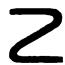
\includegraphics[keepaspectratio]{images/part002_d9406660.jpg}}

Note that if \(\mathbf{A} \neq \mathbf{K}\) then a principal fractional ideal \(\neq \{0\}\) is not an ideal of \(\mathbf{K}\) considered as a ring.

The principal fractional ideal Ax is also denoted \((x)\) . We will write \(x \equiv 0 \pmod{y}\) for \(x \in Ay\) and \(x \equiv x' \pmod{y}\) for \(x - x' \in Ay\) ; if \(x \equiv x' \pmod{y}\) then \(zx \equiv zx' \pmod{zy}\) for any \(z \in K\) .

Note that \(x \equiv x' (\bmod y)\) does not imply \(zx \equiv zx' (\bmod y)\) unless \(z \in A\) . Thus in \(\mathbf{Q}\) , relative to \(\mathbf{Z}\) , we have \(4 \equiv 2 (\bmod 2)\) but not \(2 \equiv 1 (\bmod 2)\) .

The relation \(x \mid y\) is obviously equivalent to \((x) \supset (y)\) . The mapping \(x \mapsto (x)\) from \(K^*\) onto the set \(\mathcal{P}^*\) of principal fractional ideals \(\neq (0)\) of \(K\) thus defines, on passing to the quotient, a bijective mapping from \(K^*/A^*\) onto \(\mathcal{P}^*\) ; translating the group structure of \(K^*/A^*\) to \(\mathcal{P}^*\) by means of this mapping, we are led to define the product of two principal fractional ideals \((x)\) and \((y)\) to be the ideal \((xy)\) , which depends only on \((x)\) and \((y)\) . Equipped with this law and the order relation \((x) \supset (y)\) , the set \(\mathcal{P}^*\) is an ordered group, isomorphic to \(K^*/A^*\) . By convention we will identify \(\mathcal{P}^*\) with \(K^*/A^*\) via the above map.

Note that the relation « x divides y » which, in the case of positive integers, implies that x is smaller than y, corresponds to the inclusion \((x) \supset (y)\) , in which the ideal \((x)\) is « greater » than the ideal \((y)\) . We can keep this « order reversal » in mind by noting that for example 7 has « more multiples » than 91.

If we extend the relation \(x \mid y\) to all elements of \(\mathbf{K}\) , this relation is still equivalent to \((x) \supset (y)\) in the set \(\mathcal{P}\) of all principal fractional ideals of \(\mathbf{K}\) (in which (0) is the smallest element under the relation of inclusion).

As in the previous sections, we will generally be using additive notation in the sequel. However, terminology relating to divisibility will be introduced following the corresponding additive terminology, in paragraphs preceded by the sign (DIV) (in which it is understood that the notation used is that of the present section). In order to make the reader's task easier, certain results will be translated into the language of divisibility, the translation of Prop. 7, for example, being denoted « PROPOSITION 7 (DIV) ».

\subsection{Elementary operations on ordered groups}

Let H be a subgroup of an ordered group G; it is clear that the restriction to H of the ordering of G is compatible with the group structure of H; we will always take H to be ordered in this way, unless otherwise stated. If P is the set of positive elements of G then the set of positive elements of H is \(H \cap P\) .

Let \((\mathbf{G}_{\alpha})\) be a family of ordered groups; according to the definition of the product of ordered sets (Set Theory, III, p.~137) the product group \(\mathbf{G} = \prod_{\alpha}\mathbf{G}_{\alpha}\) is

equipped with an ordering, the relation \(\ll (x_{\alpha}) \leqslant (y_{\alpha})\) between two elements of G being by definition the same as \(\ll x_{\alpha} \leqslant y_{\alpha}\) for all \(\alpha\) . It is immediate that this ordering is compatible with the group structure of G; this ordering makes G an ordered group which we call the product of the ordered groups \(G_{\alpha}\) . The positive elements of G are those elements all of whose components are positive. In the case where all the factors \(G_{\alpha}\) are identical to the same ordered group H, then G is the group \(H^{I}\) of maps from the index set I into H, the relation \(\ll f \leqslant g\) between two maps from I into H being the same as \(\ll f(\alpha) \leqslant g(\alpha)\) for all \(\alpha \in I\) ; the positive maps are those which take only positive values. The direct sum of a family \((G_{\alpha})\) of ordered groups is defined as an ordered subgroup of their product (II, p.~202).

Let \((\mathbf{G}_{\iota})_{\iota \in I}\) be a family of ordered groups whose index set I is well ordered; recall (Set Theory, III, p.~157) that an order relation, called the lexicographic ordering, is defined on the product set \(\mathbf{G} = \prod_{\iota} \mathbf{G}_{\iota}\) , the relation \(\ll (x_{\iota}) < (y_{\iota})\)

between two elements of G being by definition the same as « if β is the smallest of the indices i such that \(x_{i} \neq y_{i}\) , then \(x_{\beta} < y_{\beta}\) ». Recall that the product of a well ordered family of totally ordered sets is totally ordered under the lexicographic ordering. In the general case, the lexicographic ordering on G is compatible with its group structure, as is immediately verified; equipped with this ordering, the group G is thus an ordered group, called the lexicographic product of the well ordered family of ordered groups ( \(G_{i}\) ).

Remarks. --- 1) In the commonest cases, the well ordered index set I will be a finite interval \([1, n]\) in \(\mathbf{N}\) .

\begin{enumerate}
\def\labelenumi{\arabic{enumi})}
\setcounter{enumi}{1}
\tightlist
\item
  The set of positive elements of the lexicographic product G consists of 0 and those nonzero elements whose nonzero component of least index is positive.
\end{enumerate}

\subsection{Increasing homomorphisms of ordered groups}

Let G and \(G'\) be two ordered groups; among the homomorphisms f from the underlying additive group of G into that of \(G'\) , it makes sense to consider the increasing maps, that is those such that \(x \leqslant y\) implies \(f(x) \leqslant f(y)\) . Because of the relation \(f(y - x) = f(y) - f(x)\) it follows that the increasing homomorphisms from G into \(G'\) are characterised by the fact that the image of a positive element of G under such a homomorphism is a positive element of \(G'\) ; if P (resp. \(P'\) ) denotes the set of positive elements of G (resp. G'), this can be written \(f(P) \subset P'\) . It is clear that the canonical injection of a subgroup G into an ordered group G', and the projection of a product of ordered groups onto one of its factors, are increasing homomorphisms.

An isomorphism (VI, p.~2) f from an ordered group G onto an ordered group \(G'\) is a bijective homomorphism from G onto \(G'\) such that both f and the inverse homomorphism are increasing, in other words \(f(P) = P'\) .

It can happen that an isomorphism from the underlying group of G onto that of \(G'\) can be increasing without the inverse isomorphism also being increasing. This is the case, for example, if \(G = G'\) , if f is the identity map on G, and if \(P \subset P'\) but \(P \neq P'\) . Thus in Z we can take \(P'\) to be the set of (ordinary) positive integers and P to be the set of even positive integers.

(DIV) Let K be the field of rational functions \(\mathbf{F}_{2}(\mathbf{X})\) over the field \(F_{2}\) of order 2. The divisibility relations relative to the rings \(F_{2}[X] = A'\) and \(F_{2}[X^{2}, X^{3}] = A\) define two distinct ordered group structures on \(K^{*}\) , such that \(A \subset A'\) (they are ordered group structures since 1 is the only unit in A and the only unit in \(A'\) ).

\subsection{Suprema and infima in an ordered group}

Recall (Set Theory, III, p.~141) that if the set of upper bounds of a subset \(F\) of an ordered set \(E\) (that is to say the set of \(z \in E\) such that \(x \leqslant z\) for all \(x \in F\) ) has a least element \(a\) , then this element, which is then unique, is called the supremum of \(F\) . If \(F\) is the set of elements in a family \((x_{i})_{i \in I}\) of elements of \(E\) , its supremum, if it exists, is denoted \(\sup_{i \in I} x_i\) (or \(\sup_{i} x_i\) or simply \(\sup(x_i)\) ); if it is a

finite family \((x_{\iota})\) \((1 \leqslant \iota \leqslant n)\) , this supremum is also denoted sup \((x_{1}, \ldots, x_{n})\) . The infimum is defined in an analogous manner and is denoted inf. The operations sup and inf are associative and commutative.

Recall (Set Theory, loc. cit.) that if F is a subset of an ordered set E, and \((x_{t})\) a family of elements of F, then the existence of \(\sup(x_{t})\) in E (which may be denoted \(\sup_{E}(x_{t})\) ) does not imply the existence of a supremum of the \(x_{t}\) in F (which may be denoted \(\sup_{F}(x_{t})\) when it does exist); if both exist we know only that \(\sup_{E}(x_{t}) \leqslant \sup_{F}(x_{t})\) ; however if \(\sup_{E}(x_{t})\) exists and belongs to F, then \(\sup_{F}(x_{t})\) exists and is equal to \(\sup_{E}(x_{t})\) . For example, in the polynomial ring A = K{[}X, Y{]} (K a field), the principal ideals AX and AY have the ideal AX + AY as supremum (under the relation ⊂) in the ordered set of ideals of A, but have the ideal A as supremum in the set of all principal ideals of A.

(DIV) An element \(d\) of \(\mathbf{K}^*\) is called a greatest common divisor, or gcd for short, of a family \((x_{\iota})\) of elements of \(\mathbf{K}^*\) , if the principal fractional ideal \((d)\) is the supremum in \(\mathcal{P}^*\) (under the relation \(\subset\) ) of the family of ideals \(((x_{\iota}))\) , or in other words if the relation \(z \mid d\) for \(z \in \mathbf{K}^*\) is equivalent to \(\ll z \mid x_{\iota}\) for all \(\iota\) ». In the same way we will say that \(m \in \mathbf{K}^*\) is a least common multiple or an lcm of the family \((x_{\iota})\) if \((m)\) is the infimum in \(\mathcal{P}^*\) of the family of ideals \(((x_{\iota}))\) , that is if \(m \mid z\) is equivalent to \(\ll x_{\iota} \mid z\) for all \(\iota\) . It amounts to the same thing to say that \((m) = \bigcap_{\iota} (x_{\iota})\) ; indeed, the condition \(x_{\iota} \mid z\) for all \(\iota\) is equivalent to \(z \in Ax_{\iota}\) for all
\(\iota\) , that is to \(z \in \cap (x_{\iota})\) , and the condition \(m \mid z\) is equivalent to \(z \in (m)\) \(^{1}\) .

\pandocbounded{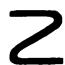
\includegraphics[keepaspectratio]{images/part002_2ca33fff.jpg}}

Note that if a principal fractional ideal \((d)\) satisfies \((d) = \sum_{i} (x_i)\) then \(d\) is a gcd of the family \((x_{\iota})\) ; but conversely a gcd of \((x_{\iota})\) does not necessarily satisfy the above condition (cf.~VI, p.~33, Ex. 24).

The gcd and lcm, if they exist, are well defined modulo the subgroup U of units of \(K^{*}\) , that is two gcd's (or two lcm's) of a given family are associate; by abuse of language we will often write \(\gcd(x_{t})\) and \(\operatorname{lcm}(x_{t})\) for any of the gcd's or lcm's of the family \((x_{t})\) , whenever such elements exist.

(DIV) By abuse of language we sometimes extend the notion of gcd to a family \((x_{i})\) of elements of K, some of which may be zero; this gcd is again defined to be an element d such that the relation \(z \mid d\) is equivalent to « \(z \mid x_{i}\) for all \(i\) »; clearly d is 0 if all the \(x_{i}\) are zero; otherwise d is a gcd of the nonzero \(x_{i}\) . Similarly the lcm of a family, some elements of which are zero, is 0.

In an ordered group G, an immediate consequence of the invariance under translation of the ordering (VI, p.~2, Prop. 2) is that

\[
\sup \left(z + x _ {i}\right) = z + \sup \left(x _ {i}\right)\tag{1}
\]

in the sense that, whenever one side is defined, then so is the other and the two are equal. Similarly, it follows from the fact that the map \(x \mapsto -x\) takes the ordering of G to the opposite ordering (VI, p.~3, Cor.) that

\[
\inf (- x _ {i}) = - (\sup (x _ {i})),\tag{2}
\]

this relation being understood in the same sense as the previous one.

PROPOSITION 6. --- Let \((x_{\alpha})_{\alpha \in A}, (y_{\beta})_{\beta \in B}\) be two families of elements of an ordered group G, each having a supremum. Then the family \((x_{\alpha} + y_{\beta})_{(\alpha, \beta) \in A \times B}\) has a supremum, and \(\sup_{(\alpha, \beta) \in A \times B} (x_{\alpha} + y_{\beta}) = \sup_{\alpha \in A} x_{\alpha} + \sup_{\beta \in B} y_{\beta}\) .

Indeed, from \(x_{\alpha} + y_{\beta} \leqslant z\) for all \(\alpha\) and \(\beta\) , we deduce \(\sup (x_{\alpha}) + y_{\beta} \leqslant z\) for all \(\beta\) , and hence \(\sup (x_{\alpha}) + \sup (y_{\beta}) \leqslant z\) .

\subsection{Lattice ordered groups}

Recall that an ordered set in which every non empty finite subset has a supremum and an infimum is called a lattice (E, III, p.~13). It is clear that a product of lattice ordered groups, and in particular a product of totally ordered groups, is a lattice ordered group. In contrast a subgroup of a lattice ordered group is not necessarily lattice ordered.

Thus, in the product ordered group \(\mathbf{Z} \times \mathbf{Z}\) , the «antidiagonal» (set of pairs \((n, n')\) such that \(n + n' = 0\) ) is ordered with the discrete ordering, and hence is not a lattice ordered group. * The additive group of polynomials in one real variable (VI, p.~1, example 2) is a filtered group (since both \(p(x)\) and \(q(x)\) are less than \((p(x))^2 + (q(x))^2 + 1\) ) which one can show is not lattice ordered. *

PROPOSITION 7. --- If \(x\) and \(y\) are two elements of an ordered group \(G\) , and if one of the elements \(\inf(x, y)\) , \(\sup(x, y)\) exists, then so does the other, and \(x + y = \inf(x, y) + \sup(x, y)\) .

Indeed, according to the relations (1) and (2) (VI, p.~9) we have

\[
\sup (a - x, a - y) = a + \sup (- x, - y) = a - \inf (x, y),
\]

and it suffices to take \(a = x + y\) .

PROPOSITION 7 (DIV). --- If \(a, b \in \mathbf{K}^{*}\) , and if \(d\) is a gcd of \(a\) and \(b\) , and \(m\) an lcm of \(a\) and \(b\) , then the product dm is an associate of \(ab\) .

PROPOSITION 8. --- Let P be the set of positive elements of an ordered group G. For G to be lattice ordered, it is necessary and sufficient that G = P - P, and that in addition P, equipped with the induced ordering, satisfies one or other of the following conditions :

\begin{enumerate}
\def\labelenumi{\alph{enumi})}
\item
  Each pair of elements of \(\mathbf{P}\) has a supremum in \(\mathbf{P}\) .
\item
  Each pair of elements of \(\mathbf{P}\) has an infimum in \(\mathbf{P}\) .
\end{enumerate}

The necessity of these conditions is obvious: indeed the relation \(G = P - P\) says that G is filtered (VI, p.~4, Prop. 4); on the other hand the supremum and infimum in G of two elements of P are positive, so are also their supremum and infimum in P.

Conversely, note first that under hypothesis a) (resp. b)), every pair of elements x, y of P has a supremum (resp. infimum) in G equal to its supremum a (resp. infimum b) in P. This is obvious for a, since any upper bound for x and y is positive; for b, let \(z \in G\) be a lower bound for x and y; then there exists \(u \in P\) such that \(z + u \in P\) , since G = P - P; now \(\inf_{P}(x + u, y + u)\) is greater than \(b + u\) , and so is of the form \(b + c + u\) ( \(c \geqslant 0\) ); since \(b + c\) is less than x and less than y, we have c = 0; hence \(\inf_{P}(x + u, y + u) = b + u\) , which implies \(z + u \leqslant b + u\) , thus \(z \leqslant b\) and b is certainly the infimum of x and y in G. Now if x and y are arbitrary elements of G we translate them into P: let \(v \in P\) be such that \(x + v\) and \(y + v\) are positive (VI, p.~5, Prop. 5); under hypothesis a) (resp. b))

there exists a supremum (resp. infimum) for \(x + v\) and \(y + v\) in P, and hence also in G by what we have just seen; by translation x and y have a supremum (resp. infimum) in G; the existence of one of these implies the other, by Prop. 7, and this shows that the conditions are sufficient.

\subsection{The decomposition theorem}

THEOREM 1 (decomposition theorem). --- Let \((x_i)_{1 \leq i \leq p}\) and \((y_j)_{1 \leq j \leq q}\) be two finite sequences of positive elements of a lattice ordered group \(G\) such that \(\sum_{i=1}^{p} x_i = \sum_{j=1}^{q} y_j\) ; then there exists a double sequence \((z_{ij})_{1 \leq i \leq p, 1 \leq j \leq q}\) of positive elements of \(G\) such that \(x_i = \sum_{j=1}^{q} z_{ij}\) for all \(i\) , and \(y_j = \sum_{i=1}^{p} z_{ij}\) for all \(j\) .

\begin{enumerate}
\def\labelenumi{\arabic{enumi})}
\tightlist
\item
  Let us prove the theorem first for the case \(p = q = 2\) . Let \(x, x', y, y'\) be positive elements of \(G\) such that \(x + x' = y + y'\) , and put \(a = \sup (0, x - y')\) . Since
\end{enumerate}

\[
x - y ^ {\prime} = y - x ^ {\prime}
\]

is less than \(x\) and less than \(y\) , it follows that \(b = x - a\) and \(c = y - a\) are positive, as is \(d = a - (x - y')\) . Also we have

\[
x = a + b, x ^ {\prime} = c + d, y = a + c \quad \text { and } \quad y ^ {\prime} = b + d.
\]

\begin{enumerate}
\def\labelenumi{\arabic{enumi})}
\setcounter{enumi}{1}
\tightlist
\item
  Let us now show that if the theorem is true for \(p < m\) and \(q = n\) ( \(m > 2\) , \(n \geqslant 2\) ) then it is true for \(p = m\) and \(q = n\) . By hypothesis we have \(x_{m} + \sum_{i=1}^{m-1} x_{i} = \sum_{j=1}^{n} y_{j}\) . The theorem being true for \(p = 2\) and \(q = n\) , there exist two finite sequences \((z_{j}')\) , \((z_{j}''')\) of \(n\) positive terms such that \(\sum_{i=1}^{m-1} x_{i} = \sum_{j=1}^{n} z_{j}'\) , \(x_{m} = \sum_{j=1}^{n} z_{j}''\) , and \(y_{j} = z_{j}' + z_{j}''\) for \(1 \leqslant j \leqslant n\) . On the other hand, since the theorem is true for \(p = m-1\) and \(q = n\) , there exists a double sequence \((u_{ij})_{1 \leqslant i \leqslant m-1, 1 \leqslant j \leqslant n}\) such that \(x_{i} = \sum_{j=1}^{n} u_{ij}\) for \(1 \leqslant i \leqslant m-1\) , and \(z_{j}' = \sum_{i=1}^{m-1} u_{ij}\) for \(1 \leqslant j \leqslant n\) . Putting
\end{enumerate}

\[
z _ {i j} = u _ {i j} \quad \text { for } \quad 1 \leqslant i \leqslant m - 1, \quad \text { and } \quad z _ {m j} = z _ {j} ^ {\prime \prime} \quad (1 \leqslant j \leqslant n),
\]

we certainly obtain a double sequence satisfying the conditions of the theorem. 3) By interchanging the \(x_{i}\) and the \(y_{j}\) we see in the same way that, if the theorem is true for \(p = m\) and \(q < n\) ( \(m \geqslant 2\) , \(n > 2\) ), then it is true for \(p = m\) and \(q = n\) . The theorem is thus proved by double induction starting from the case \(p = q = 2\) , for it is trivially true whenever \(p \leqslant 1\) or \(q \leqslant 1\) .

COROLLARY. --- Let \(y, x_1, x_2, \ldots, x_n\) be \(n + 1\) positive elements of \(G\) such that \(y \leqslant \sum_{i=1}^{n} x_i\) ; then there exist \(n\) positive elements \(y_i (1 \leqslant i \leqslant n)\) such that \(y_i \leqslant x_i\) and \(y = \sum_{i=1}^{n} y_i\) .

It is sufficient to apply theorem 1 to the sequence \((x_{i})\) and the sequence consisting of the two elements \(y\) and \(z = \left(\sum_{i=1}^{n} x_{i}\right) - y\) .

\subsection{Positive and negative parts}

DEFINITION 4. --- In a lattice ordered group G the positive part (resp. negative part, absolute value) of an element \(x \in G\) is the element \(\sup(x, 0)\) (resp. \(\sup(-x, 0)\) , \(\sup(x, -x)\) ), which is denoted \(x^{+}\) (resp. \(x^{-}\) , \(|x|\) ).

\pandocbounded{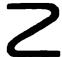
\includegraphics[keepaspectratio]{images/part002_7ee71349.jpg}}

Despite its name, the negative part \(x^{-}\) is a positive element.

Clearly \(x^{-} = (-x)^{+}\) and \(|-x| = |x|\) . Let us also note the following formulae, the first of which is an immediate consequence of the definitions and of the invariance of the ordering under translation, and the second of which follows from the first by Prop. 7 of VI, p.~10:

\[
\left\{ \begin{array}{l} \sup (x, y) = x + (y - x) ^ {+}, \\ \inf (x, y) = y - (y - x) ^ {+}. \end{array} \right.\tag{3}
\]

PROPOSITION 9. --- a) For each element x of a lattice ordered group G we have \(x = x^{+} - x^{-}\) and \(\inf(x^{+}, x^{-}) = 0\) .

\begin{enumerate}
\def\labelenumi{\alph{enumi})}
\setcounter{enumi}{1}
\item
  For every expression of \(x\) as the difference of two positive elements, say \(x = u - v\) , we have \(u = x^{+} + w\) and \(v = x^{-} + w\) with \(w = \inf(u, v)\) . In particular if \(\inf(u, v) = 0\) then \(u = x^{+}\) and \(v = x^{-}\) .
\item
  The relation \(\ll x\leqslant y\gg\) is equivalent to \(\ll x^{+}\leqslant y^{+}\) and \(x^{-}\geqslant y^{-}\gg\) .
\item
  We have \(|x| = x^{+} + x^{-} \geqslant 0\) .
\item
  For any \(x\) and \(y\) in \(G\) , we have the inequality \(|x + y| \leqslant |x| + |y|\) , and more generally \(\left|\sum_{i=1}^{n} x_i\right| \leqslant \sum_{i=1}^{n} |x_i|\) for any finite family \((x_i)\) of elements of \(G\) .
\item
  For any \(x\) and \(y\) in \(G\) we have \(||x| - |y|| \leqslant |x - y|\) .
\end{enumerate}

We will prove \(a)\) and \(b)\) simultaneously. If \(x = u - v\) with \(u\) and \(v\) positive, then \(u \geqslant x\) , so \(u \geqslant \sup (x, 0) = x^{+}\) , and \(w = u - x^{+}\) is positive. On the other hand we have

\[
x ^ {+} - x = \sup (x, 0) - x = \sup (x - x, - x) = x ^ {-}
\]

from which it follows that \(x = x^{+} - x^{-}\) , and \(v - x^{-} = w\) . If \(z \leqslant x^{-}\) then \(z \leqslant x^{+} - x\) , and so \(x \leqslant x^{+} - z\) ; if also \(z \leqslant x^{+}\) , then \(x^{+} - z\) is positive, and so \(x^{+} \leqslant x^{+} - z\) by definition of \(x^{+}\) . Hence we have \(z \leqslant 0\) , which implies \(\inf(x^{+}, x^{-}) = 0\) , whence by translation \(\inf(u, v) = w\) .

\begin{enumerate}
\def\labelenumi{\alph{enumi})}
\setcounter{enumi}{2}
\item
  The relation \(x \leqslant y\) implies \(\sup (y, 0) \geqslant x\) and \(\sup (y, 0) \geqslant 0\) , hence \(x^{+} \leqslant y^{+}\) ; similarly if \(-y \leqslant -x\) we deduce \(x^{-} \geqslant y^{-}\) . The converse implication follows immediately from \(x = x^{+} - x^{-}\) and \(y = y^{+} - y^{-}\) .
\item
  Since \(x \leqslant x^{+}\) and \(-x \leqslant x^{-}\) , it is clear that
\end{enumerate}

\[
\left| x \right| = \sup (x, - x) \leqslant x ^ {+} + x ^ {-}.
\]

Conversely, if \(a \geqslant x\) and \(a \geqslant -x\) then we deduce from \(c\) ) that \(a^+ \geqslant x^+\) , \(a^+ \geqslant x^-\) , \(a^- \leqslant x^-\) and \(a^- \leqslant x^+\) ; since \(a^-\) is positive and \(\inf(x^+, x^-) = 0\) , the last two inequalities imply \(a^- = 0\) and \(a = a^+\) ; the first two inequalities then give \(a \geqslant \sup(x^+, x^-)\) , and \(\sup(x^+, x^-)\) is equal to \(x^+ + x^-\) by \(a\) ) and by Prop. 7 of VI, p.~10.

\begin{enumerate}
\def\labelenumi{\alph{enumi})}
\setcounter{enumi}{4}
\item
  Since \(x \leqslant |x|\) and \(y \leqslant |y|\) , we have \(x + y \leqslant |x| + |y|\) ; since \(-x \leqslant |x|\) and \(-y \leqslant |y|\) , we have \(-x - y \leqslant |x| + |y|\) ; whence the first inequality. The second follows by induction on \(n\) .
\item
  Replacing \(x\) and \(y\) by \(y\) and \(x - y\) in \(e\) ), we obtain
\end{enumerate}

\[
\left| x \right| - \left| y \right| \leqslant \left| x - y \right|;
\]

similarly we have \(|y| - |x| \leqslant |y - x| = |x - y|\) ; whence the stated result.

Remark. --- We deduce from \(d\) that \(|x|=0\) implies \(x=0\) (for \(x^{+}\) and \(x^{-}\) are positive); thus \(x\neq0\) implies \(|x|>0\) .

PROPOSITION 9 (DIV). --- If the group \(\mathcal{P}^*\) of principal fractional ideals of K is lattice ordered, then every element \(x\) of \(\mathbf{K}^*\) can be written in the form \(x = uv^{-1}\) , where \(u\) and \(v\) are elements of A such that \(1 = \gcd(u, v)\) ; for any other expression \(x = u'v'^{-1}\) of \(x\) as the quotient of two elements of A, we have \(u' = uw\) and \(v' = vw\) , where \(w\) is a gcd of \(u'\) , \(v'\) ; in particular if \(1 = \gcd(u', v')\) then \(u'\) and \(v'\) are associates of \(u\) and \(v\) respectively.

Such an expression \(uv^{-1}\) for an element x of \(K^{*}\) is often called a reduced fraction.

\subsection{Coprime elements}

DEFINITION 5. --- In an ordered group two elements x and y are called coprime if \(\inf(x, y) = 0\) .

In some cases it is natural to define two elements to be coprime if \(\inf(|x|, |y|) = 0\) (cf.~INT, II, § 1) or to introduce the corresponding terminology in divisibility theory. We shall not do so here.

Two coprime elements are necessarily positive. The positive and negative parts \(x^{+}\) and \(x^{-}\) of x are coprime (VI, p.~12, Prop. 9, a)). The elements \(x_{i}\) of a family \((x_{t})_{t\in I}\) are said to be setwise coprime if \(\inf_{t\in I}x_t = 0\) ; if the \(x_{t}\) are all \(\geqslant 0\) then it is

sufficient for there to exist a finite subset J of I such that the corresponding elements are setwise coprime. The elements of a family \((x_{\iota})\) are said to be pairwise coprime if \(\inf(x_{\iota}, x_{\kappa}) = 0\) for every pair \((\iota, \kappa)\) of distinct indices.

The \(x_{i}\) can be setwise coprime without being pairwise coprime.

If \(x\) and \(y\) are coprime, we also say that \(x\) is coprime to \(y\) , or that \(y\) is coprime to \(x\) .

(DIV) Two elements x and y of K are said to be coprime if the principal ideals \((x)\) and \((y)\) are nonzero and coprime in \(P^{*}\) ; this amounts to saying that 1 is a gcd of x and y, and implies that x and y belong to A. For example the numerator and denominator of a reduced fraction are coprime. The notions of pairwise and setwise coprime elements are defined similarly.

(DIV) When \(x\) and \(y\) are coprime, they are often said to be « prime to one another »; it is convenient to avoid this terminology, which can lead to confusion with the notion of prime numbers (I, p.~50, Def. 16).

PROPOSITION 10. --- Let \(x, y\) and \(z\) be three elements of an ordered group; for \(x - z\) and \(y - z\) to be coprime, it is necessary and sufficient that \(z = \inf(x, y)\) .

Indeed the relations \(z = \inf (x, y)\) and \(0 = \inf (x - z, y - z)\) are equivalent.

PROPOSITION 10 (DIV). --- Let \(a, b\) and \(c\) be three elements of \(\mathbf{K}\) with \(c \neq 0\) ; for the quotients \(ac^{-1}\) and \(bc^{-1}\) to be coprime, it is necessary and sufficient that \(c\) be a gcd of \(a\) and \(b\) .

PROPOSITION 11. --- If \((x_{i})\) , \((y_{j})\) are two finite families of positive elements of a lattice ordered group, then

\[
\inf \left(\sum_ {i} x _ {i}, \sum_ {j} y _ {j}\right) \leqslant \sum_ {i, j} \inf (x _ {i}, y _ {j}).
\]

Arguing by induction on the number of elements in the families \((x_{i})\) and \((y_{j})\) , it is enough to prove that, if \(x, y\) and \(z\) are positive elements, then

\[
\inf (x, y + z) \leqslant \inf (x, y) + \inf (x, z).
\]

Indeed, put \(t = \inf(x, y + z)\) ; by VI, p.~12, Cor., we can write \(t = t_1 + t_2\) with \(0 \leqslant t_1 \leqslant y\) and \(0 \leqslant t_2 \leqslant z\) ; since \(t_1\) and \(t_2\) are positive, we also have \(t_1 \leqslant x\) and \(t_2 \leqslant x\) , whence \(t_1 \leqslant \inf(x, y)\) and \(t_2 \leqslant \inf(x, z)\) .

COROLLARY 1. --- If x and y are two coprime elements, and z a positive element, of a lattice ordered group, then \(\inf(x, z) = \inf(x, y + z)\) .

Indeed \(\inf (x,y + z)\leqslant \inf (x,z)\) by Prop. 11, and \(\inf (x,z)\leqslant \inf (x,y + z)\) since \(y\geqslant 0\) , whence the corollary.

COROLLARY 2. --- In a lattice ordered group, if x and y are coprime and if \(z \geqslant 0\) and \(x \leqslant y + z\) , then \(x \leqslant z\) .

COROLLARY 3. --- In a lattice ordered group, if x is coprime to y and to z, then it is also coprime to \(y + z\) .

COROLLARY 4. --- If \((x_i)_{1 \leq i \leq n}\) and \((y_j)_{1 \leq j \leq m}\) are two finite families of elements of a lattice ordered group G, such that each \(x_i\) is coprime to each \(y_j\) , then \(x_1 + \cdots + x_n\) is coprime to \(y_1 + \cdots + y_m\) .

This follows from Cor. 3 by induction on m and n.

COROLLARY 5. --- For any integer \(n \geqslant 0\) we have \((nx)^+ = nx^+\) and \((nx)^- = nx^-\) ; for all \(n \in \mathbf{Z}\) we have \(|nx| = |n| \cdot |x|\) .

Indeed \(nx = nx^{+} - nx^{-}\) ; since \(x^{+}\) and \(x^{-}\) are coprime, so are \(nx^{+}\) and \(nx^{-}\) if \(n \geqslant 0\) (Cor. 4); the first assertion follows by Prop. 9 b) of VI, p.~12. The second follows from the first by Prop. 9 d) in the case \(n \geqslant 0\) ; the case \(n < 0\) follows from this as a result of the relation \(|-x| = |x|\) .

PROPOSITION 11 (DIV). --- Suppose the set \(\mathcal{P}^*\) is a lattice, and let \((a_i)\) , \((b_j)\) be two finite families of elements of A. Then every gcd of \(\prod_{i} a_i\) and

\(\prod_{j} b_{j}\) divides the product \(\prod_{i,j} \gcd(a_{i}, b_{j})\) .

COROLLARY 1 (DIV). --- If a, b, c are three elements of A such that a is coprime to b, then every gcd of a and c is also a gcd of a and bc.

COROLLARY 2 (DIV) (Euclid's lemma). --- Let \(a, b, c\) be three elements of A. If \(a\) is coprime to \(b\) and divides \(bc\) , then it divides \(c\) .

COROLLARY 3 (DIV). --- If x is coprime to y and to z, then it is coprime to yz.

COROLLARY 4 (DIV). --- If \((x_{i})\) and \((y_{j})\) are two finite families of elements of A such that each \(x_{i}\) is coprime to each \(y_{j}\) , then the product of the \(x_{i}\) is coprime to the product of the \(y_{j}\) .

COROLLARY 5 (DIV). --- If \(d\) is a gcd of \(x\) and \(y\) , then \(d^n\) is a gcd of \(x^n\) and \(y^n\) for each positive integer \(n\) .

Indeed \(xd^{-1}\) and \(yd^{-1}\) are coprime (Prop. 10 (DIV)), and hence so are \(x^{n}d^{-n}\) and \(y^{n}d^{-n}\) (Cor. 4).

PROPOSITION 12. --- Let \(x_{i}\) ( \(1 \leqslant i \leqslant n\) ) be \(n\) pairwise coprime elements in a lattice ordered group. Then

\[
\sup \left(x _ {1}, \dots , x _ {n}\right) = x _ {1} + \dots + x _ {n}.
\]

This follows from the formula \(u + v = \sup(u, v) + \inf(u, v)\) (VI, p.~10, Prop. 7) by induction on n, using the fact that \(x_{i}\) is coprime to \(x_{1} + \cdots + x_{i-1}\) for \(2 \leqslant i \leqslant n\) (Cor. 4 to Prop. 11).

Remark. --- Prop. 7 of VI, p.~10 also shows that a necessary and sufficient condition for \(x\) and \(y\) to be coprime is that \(x + y = \sup(x, y)\) .

PROPOSITION 12 (DIV). --- Let \(a_i\) be a finite number \(n\) of pairwise coprime elements of \(A\) ; then the product \(a_1 \ldots a_n\) is an lcm of \(a_1, \ldots, a_n\) .

PROPOSITION 13. --- In a lattice ordered group G, let \((x_{\alpha})\) be a family having an infimum (resp. supremum), and let z be an arbitrary element of G; then the family \((\sup(z, x_{\alpha}))\) (resp. \((\inf(z, x_{\alpha})))\) has an infimum (resp. supremum) and

\[
\left\{ \begin{array}{l} \inf _ {\alpha} (\sup (z, x _ {\alpha})) = \sup \left(z, \inf _ {\alpha} x _ {\alpha}\right) \\ \sup _ {\alpha} (\inf (z, x _ {\alpha})) = \inf \left(z, \sup _ {\alpha} x _ {\alpha}\right) \end{array} \right.\tag{4}
\]

respectively.

Suppose that the family \((x_{\alpha})\) has an infimum \(y\) . We will show that \(\sup (z,y)\) is an infimum of the family \((\sup (z,x_{\alpha}))\) .

Indeed \(\sup (z, x_{\alpha}) = z + (x_{\alpha} - z)^{+}\) and by translating we can reduce to the case \(z = 0\) , that is we must show that \((x_{\alpha}^{+})\) has an infimum equal to \(y^{+}\) . Since \(y \leqslant x_{\alpha}\) we have \(y^{+} \leqslant x_{\alpha}^{+}\) for all \(\alpha\) (VI, p.~12, Prop. 9, c)). Conversely, if \(a \leqslant x_{\alpha}^{+}\) for all \(\alpha\) , then it follows that \(a \leqslant x_{\alpha} + x_{\alpha}^{-}\) (Prop. 9, a)); now \(y^{-} \geqslant x_{\alpha}^{-}\) since \(y \leqslant x_{\alpha}\) ; hence \(a \leqslant x_{\alpha} + y^{-}\) for all \(\alpha\) , that is \(a \leqslant y + y^{-} = y^{+}\) .

The other formula follows by changing to the opposite order relation.

COROLLARY. --- If an element z of a lattice ordered group G is coprime to each element \(x_{\alpha}\) of a family having an infimum y, then z is coprime to y.

This is an immediate consequence of the second formula (4).

Remark. --- Applying the formulae of Prop. 13 to a family of two elements \((x, y)\) , we obtain the following formulae, which express the fact that each of the laws of composition sup, inf in a lattice ordered group is distributive with respect to the other :

\[
\begin{array}{l} \sup (z, \inf (x, y)) = \inf (\sup (z, x), \sup (z, y)) \\ \inf (z, \sup (x, y)) = \sup (\inf (z, x), \inf (z, y)). \end{array}
\]

This distributivity property is peculiar to lattice ordered groups, and does not extend to arbitrary lattices, or even to lattice ordered monoids (cf.~VI, p.~33, Ex. 24).
